\documentclass{article}
\usepackage[utf8]{inputenc}
\usepackage{multicol}
\usepackage[a4paper]{geometry}
\usepackage{color}
\usepackage{mathtools}
\usepackage{amsfonts}
\usepackage{xcolor}
\usepackage{amsmath}
\usepackage{todonotes}
\usepackage[font=small,labelfont=bf]{caption}
\usepackage[hungarian]{babel}
\usepackage[T1]{fontenc} % search working after this

\title{Ipari informatika - IMSc feladat - 2022 őszi félév}
\author{Vörös Asztrik}
\date{}

\begin{document}
\maketitle

%\abstract{}
\newcommand{\dunderline}[1]{\underline{\underline{#1}}}
\newcommand{\zeros}[2]{\dunderline{0}_{#1 \times #2}}
\newcommand{\zerosV}[2]{\underline{0}_{#1 \times #2}}
\newcommand{\ZerosV}{\underline{0}}
\newcommand{\ZerosM}{\dunderline{0}}
\newcommand{\eye}[1]{\dunderline{I}_{#1 \times #1}}
\newcommand{\Eye}{\dunderline{I}}
\renewcommand{\vec}[1]{\underline{#1}}

\setlength\parindent{0pt}

\section{Rendszer - folytonos idő}
	A feladat által megadott egyenletrendszer: \\
	\begin{align}
		\begin{bmatrix}
			m+M & mL_0 & 0 \\
			m   & mL_0 & 0 \\
			0   & 0	& m+J/\rho^2
		\end{bmatrix}
		\begin{pmatrix}
			\ddot{r} \\
			\ddot{\vartheta} \\
			\ddot{l}
		\end{pmatrix}
		=
		\begin{pmatrix}
			f \\
			-mg\vartheta \\
			-\tau/\rho
		\end{pmatrix}
	\end{align}
	\\
	Ezt két egymástól független rendszerre tudjuk bontani, ahol az első rendszer feladata
	$r$-t meghatározni, míg a másiké $\vartheta$-t. Első lépésnek $x' = A x + Bu$ alakra fogom hozni az egyenleteket (a két bemenet $f$ és $\tau$). Ezután eltűntetem a kétszeres deriváltakat új változók bevezetésével.
	\\
	\subsection{$r$ rendszer}
		\begin{align}
			\begin{bmatrix}
				m+M & mL_0 \\
				m   & mL_0
			\end{bmatrix}
			\begin{pmatrix}
				\ddot{r} \\
				\ddot{\vartheta}
			\end{pmatrix}
			&=
			\begin{pmatrix}
				f \\
				-mg\vartheta
			\end{pmatrix} \\
			%
			& =
			\begin{bmatrix}
				0 & 0 \\
				0 & -mg
			\end{bmatrix}
			\begin{pmatrix}
				r \\
				\vartheta
			\end{pmatrix}
			+
			\begin{bmatrix}
				1 \\
				0
			\end{bmatrix}
			f \\
			%
			\begin{pmatrix}
				\ddot{r} \\
				\ddot{\vartheta}
			\end{pmatrix}
			& =
			\begin{bmatrix}
				m+M & mL_0 \\
				m   & mL_0
			\end{bmatrix}^{-1}
			\begin{bmatrix}
				0 & 0 \\
				0 & -mg
			\end{bmatrix}
			\begin{pmatrix}
				r \\
				\vartheta
			\end{pmatrix}
			+
			\begin{bmatrix}
				m+M & mL_0 \\
				m   & mL_0
			\end{bmatrix}^{-1}
			\begin{bmatrix}
				1 \\
				0
			\end{bmatrix}
			f \\
			%
			& \eqqcolon
			A'
			\begin{pmatrix}
				r \\
				\vartheta
			\end{pmatrix}
			+
			B'
			f
		\end{align}
        \begin{align}
			%
			\begin{pmatrix}
				\dot{x_1} = \dot{r} \\
				\dot{x_2} = \dot{\vartheta} \\
				\dot{x_3} = \ddot{r} \\
				\dot{x_4} = \ddot{\vartheta}
			\end{pmatrix}
			& =
			\begin{bmatrix}
				\zeros{2}{2} & \eye{2} \\
				A' & \zeros{2}{2}
			\end{bmatrix}
			\begin{pmatrix}
				x_1 = r \\
				x_2 = \vartheta \\
				x_3 = \dot{r} \\
				x_4 = \dot{\vartheta}
			\end{pmatrix}
			+
			\begin{bmatrix}
				\zerosV{2}{1} \\
				B'
			\end{bmatrix}
			f \\
			%
			y & =
			\begin{bmatrix}
				1 & \zerosV{1}{3} 
			\end{bmatrix}
			\begin{pmatrix}
				x_1 = r \\
				x_2 = \vartheta \\
				x_3 = \dot{r} \\
				x_4 = \dot{\vartheta}
			\end{pmatrix}
			+
			0f \\
			%
			\dot{\vec{x}} & = A_1 \vec{x} + B_1 f \\
			y & = C_1 \vec{x} + D_1f
		\end{align}
	\subsection{$l$ rendszer}
		\begin{align}
			\begin{bmatrix}
				m+J/\rho^2
			\end{bmatrix}
			\begin{pmatrix}
				\ddot{l}
			\end{pmatrix}
			&=
			\begin{pmatrix}
				-\tau/\rho
			\end{pmatrix} \\
			%
			& =
			\begin{bmatrix}
				0
			\end{bmatrix}
			\begin{pmatrix}
				l
			\end{pmatrix}
			+
			\begin{bmatrix}
				-1/\rho
			\end{bmatrix}
			\tau \\
			\begin{pmatrix}
				\ddot{l}
			\end{pmatrix}
			& =
			\begin{bmatrix}
				m+J/\rho^2
			\end{bmatrix}^{-1}
			\begin{bmatrix}
				0
			\end{bmatrix}
			\begin{pmatrix}
				l
			\end{pmatrix}
			+
			\begin{bmatrix}
				m+J/\rho^2
			\end{bmatrix}^{-1}
			\begin{bmatrix}
				-1/\rho
			\end{bmatrix}
			\tau \\
			%
			& \eqqcolon
			A'
			\begin{pmatrix}
				l
			\end{pmatrix}
			+
			B'
			\tau
        \end{align}
        \begin{align}
			\begin{pmatrix}
				\dot{x_1} = \dot{l} \\
				\dot{x_2} = \ddot{l}
			\end{pmatrix}
			& =
			\begin{bmatrix}
				\zeros{1}{1} & \eye{1} \\
				A' & \zeros{1}{1}
			\end{bmatrix}
			\begin{pmatrix}
				x_1 = l \\
				x_2 = \dot{l}
			\end{pmatrix}
			+
			\begin{bmatrix}
				\zerosV{1}{1} \\
				B'
			\end{bmatrix}
			\tau \\
			%
			y & =
			\begin{bmatrix}
				1 & \zerosV{1}{1} 
			\end{bmatrix}
			\begin{pmatrix}
				x_1 = l \\
				x_2 = \dot{l}
			\end{pmatrix}
			+
			0\tau \\
			%
			\dot{\vec{x}} & = A_2 \vec{x} + B_2 \tau \\
			y & = C_2 \vec{x} + D_2\tau
		\end{align}
\section{Domináns pólusok}
	\newcommand{\sdom}{s_{\textrm{dominant}}}
	\newcommand{\sdoms}{s_{\textrm{dominant}_{1,2}}}
	\newcommand{\re}[1]{\Re\{#1\}}
	\newcommand{\im}[1]{\Im\{#1\}}

	\begin{center}
		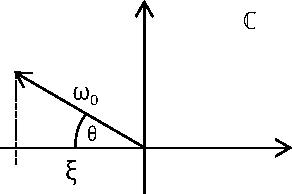
\includegraphics{asset/dominant.pdf}
	\end{center}

	A $\theta$ definíciója miatt a $\cos{\theta}$ pont $-1$-szeresét adja a komplex szám valós részének, tehát

	\begin{equation}
		\re{\sdom} = -\omega_0\xi
	\end{equation}

	Mivel a feladat paraméterezése $\xi$-t adta meg, így bár $\re{\sdom}$ egyértelmű $\im{\sdom}$ viszont nem (feltétlen) az, hiszen egy megoldás konjugáltja is azonos $\cos{\theta} \eqqcolon \xi$ értékkel fog rendelkezni.
	
	\begin{align}
		\im{\sdoms} & = \omega_0\sin{\theta} \\
		\sin^2{\theta} + \cos^2{\theta} & = 1 \\
		\sin{\theta} & = \pm \sqrt{1 - \cos^2{\theta}} \\
		\sin{\theta} & = \pm \sqrt{1 - \xi^2} \\
		\im{\sdoms} & = \pm \omega_0 \sqrt{1 - \xi^2}
	\end{align}

	Tehát

	\begin{align}
		\sdoms = -\omega_0\xi \pm \omega_0 \sqrt{1 - \xi^2}
	\end{align}
\section{Shannon kritérium}
    \newcommand{\soinf}{{s_o}_{\infty}}
    \newcommand{\scinf}{{s_c}_{\infty}}

	\begin{align}
		f_{1,2} & \coloneqq 5 \max_{ \lambda_i \in \lambda(cA_{1,2}) } | \lambda_i | \\
		%
		& =
		5 |\soinf| \\
		%
		T & \coloneqq 1/f
	\end{align}

\section{Diszkretizálás}
	Matlabban a folytonos rendszert a $c2d$ paranccsal lehet átalakítani diszkrét rendszerré, megadva a $T$ mintavételezési időt. Így az $r$ rendszert a $(\Phi_1, \Gamma_1, C_1, D_1)$ 4-es, míg az $l$ rendszert a $(\Phi_2, \Gamma_2, C_2, D_2)$ 4-es írja le.

	Az előírt sajátértékeket a következő képlettel transzformáltam át:
	\begin{align}
		z = e^{s T}
	\end{align}

    \newcommand{\zoinf}{ {{z_o}_{\infty}} }
    \newcommand{\zcinf}{ {{z_c}_{\infty}} }
	\newcommand{\zdom}{ {z_{\textrm{dominant}}} }
    Így a következő új változók jönnek létre: $\zdom_{1,2}, \zoinf, \zcinf$

\section{Stabilitás}
	Diszkrét időben a stabilitását olyan komplex számok teljesítik melyeknek a hossza kisebb mint 1. A két rendszert megvizsgálva a következő sajátértékek adódtak, így a rendszerünk labilis:
	\begin{align}
		\vec{\lambda}_r & =
		\begin{pmatrix}
			1 \\
			1 \\
			0.9938 + 0.1109i \\
			0.9938 - 0.1109i
		\end{pmatrix} 
        \\
        %
		\vec{\lambda}_l & =
		\begin{pmatrix}
			1 \\
			1
		\end{pmatrix} 
	\end{align}

    Az elkövetkező rendszerek során eltekintünk az alapjeltől, hogy az adott megoldás lényege látszódjon csak, illetve az utolsó rendszer esetén az alapjel bevezetésének módja egyértelműen alkalmazható az azelőtti rendszerekre. A képeken a $r$ rendszerek változatai fognak szerepelni, míg az egyenletek során rendszer független alakok kerülnek bemutatásra.

\section{Stabilizálás - $\vec{x}$ ismeret}
    Tekintsük az alábbi konstrukciót, ahol a rendszer bemenete $-Kx$ lesz:
    
    \begin{center}
        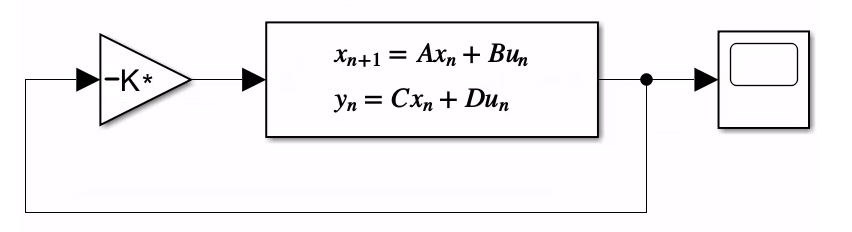
\includegraphics[width=\linewidth/2]{asset/K.png}
    \end{center}

    Ekkor a rendszerünk állapotegyenlete a következő lesz:
    
    \begin{align}
        \vec{x}_{k+1} & = \Phi \vec{x_k} + \Gamma (-K \vec{x_k}) \\
        & =
        (\Phi - \Gamma K)\vec{x_k}     
    \end{align}

    Látható, hogy az új rendszer $\Phi$ mátrixa $\Phi - \Gamma K$ lesz, ahol $K$-t mi választjuk meg. Az Ackermann képlet segítségével megfelelő sajátértékek megválasztásával megkaphatjuk a $K$ mátrixot. Ehhez azonban az kell, hogy a rendszer irányítható legyen, azaz létezzen az ${M_c}_{1,2}^{-1}$, amit Matlabban a $ctrb$ és a $rank$ függvények segíségével tudunk megállapítani.    
    
    Mivel a két rendszer irányítható, így a feladat kiírása szerint a következő sajátértékek írjuk elő a rendszer számára:

    \begin{align}
		\vec{\lambda}_r & =
		\begin{pmatrix}
			\zdom_1 \\
			\zdom_2 \\
			\zoinf \\
			\zoinf
		\end{pmatrix} 
        \\
        %
		\vec{\lambda}_l & =
		\begin{pmatrix}
			\zdom_1 \\
			\zdom_2
		\end{pmatrix} 
    \end{align}

\section{Stabilizálás - $\vec{x}$ ismeretlen}
    Mivel az állapotváltozó ismeretének számos akadálya lehet, ezért egy becslőt alkalmazunk annak megállapítására, felhasználva a rendszer kimenetét és bemenetét.

    \begin{center}
        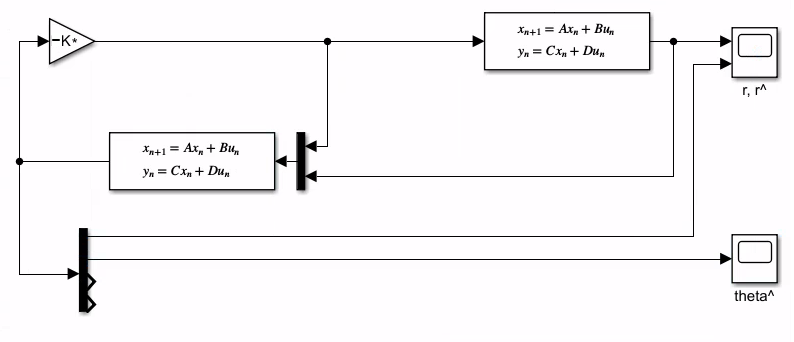
\includegraphics[width=\linewidth]{asset/x^.png}
    \end{center}

    Az állapotmegfigyelő állapotegyenelete a következő ($D = 0$-t feltételezve):
    \begin{align}
        x_{k+1}^{\textrm{becslő}} \eqqcolon \hat{x}_{k+1} & = \Phi \hat{x}_k + \Gamma u_k + G { { y_{\textrm{eltérés}} }_{k+1} } \\
        & = \Phi \hat{x}_k + \Gamma u_k + G(y_{k+1} - \hat{y}_{k+1}^{rendszer}) \\
        & = \Phi \hat{x}_k + \Gamma u_k + G(y_{k+1} - C\hat{x}_{k+1}^{renszer}) \\
        & = \Phi \hat{x}_k + \Gamma u_k + G(y_{k+1} - C(\Phi \hat{x}_k + \Gamma u_k)) \\
        & = (\Phi - GC\Phi)\hat{x}_k + (\Gamma - GC\Gamma) u_k + Gy_{k+1} \\
        & = F\hat{x}_k + Hu_k + Gy_{k+1} \\
        & = F\hat{x}_k + 
        \begin{bmatrix}
            H & G
        \end{bmatrix}
        \begin{pmatrix}
            u_k \\
            y_{k+1}
        \end{pmatrix} \\
        & = F \hat{x}_k + H'u'_k
    \end{align}
    \begin{align}
        y_k^{\textrm{becslő}} & = \Eye \hat{x}_k + \ZerosV u'_k
    \end{align}
    A rendszer sajátértékeit $F = (\Phi - GC)$ tartalmazza, amiket $G$ erősítési mátrix segítségével tudunk megválasztani, célszerűen gyorsabb csillapítással, mint az állapotvisszacsatolás esetén. A feladat által megjelölt sajátértékek:
    \begin{align}
		\vec{\lambda}_r & = \{\zoinf\}^4 \\
		\vec{\lambda}_l & = \{\zoinf\}^2 
    \end{align}
    Az Ackermann képlethez azonban $Q - WG$ alakra van szükségünk:
    \begin{align}
        (\Phi - GC\Phi)^T & = \Phi^T - \Phi^T C^T G^T \\
        & = Q - WG^T
    \end{align}
    Ezzel az átrendezéssel tehát meg tudjuk határozni $G^T$-t, ha a becslő megfigyelhető, azaz létezik ${M_o^T}_{1,2}^{-1}$, amit Matlabban a $obsv$ és a $rank$ függvények segíségével tudunk megállapítani. $G^T$-t transzponálvas ezek után megkapjuk $G$-t.  

\section{Terhelés és Terhelésbecslő}
    \subsection{Terhelés}
        Előfordulhat, hogy az általunk meghatározott rendszer bementet zaj éri és azt megakadályozni, illetve megfigyelni nem tudjuk. Ha a zaj elég hosszú kiterjedésű intervallumokra bontható, amiken belül konstans értékeket vesz fel, akkor azt meg tudjuk becsülni.

        \begin{center}
            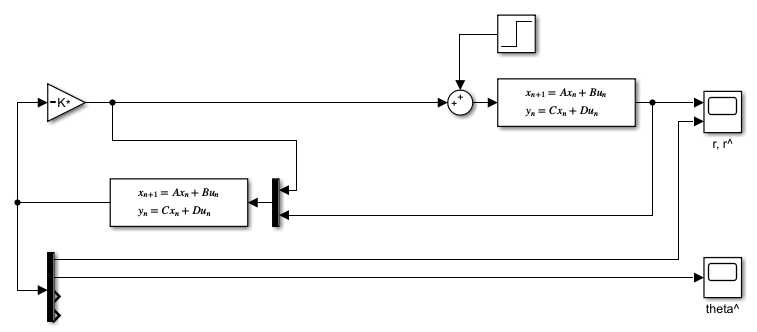
\includegraphics[width=\linewidth]{asset/d.png}
        \end{center}
        
        A becslést úgy tehetjük meg, hogy a zajt a rendszer részeként tekintjük, hiszen befolyásolni és mérni nem tudjuk közvetlenül. Azaz a rendszer állapotvektorát kibővítjük a zaj jelenlegi értékével $d$-vel. Az állapotegyenlet felírásakor felhasználjuk azt a tényt, hogy adott intervallumon belül a zaj konstans, így $d_{k+1} = d_k$, illetve $D$-t most is 0-nak tekintjük.

        \begin{align}
            \begin{pmatrix}
                x_{k+1} \\
                d_{k+1}
            \end{pmatrix}
            & =
            \begin{bmatrix}
                \Phi & \Gamma \\
                \vec{0} & 1
            \end{bmatrix}
            \begin{pmatrix}
                x_k \\
                d_k
            \end{pmatrix}
            +
            \begin{bmatrix}
                \Gamma \\
                0
            \end{bmatrix}
            u_k \\
            %
            y_k & =
            \begin{bmatrix}
                C & 0
            \end{bmatrix}
            \begin{pmatrix}
                x_k \\
                d_k
            \end{pmatrix}
        \end{align}
        
        Bevezetve új változókat az így kapott rendszer állapotegyenelete:
        \newcommand{\tx}{\tilde{x}}
        \newcommand{\tPhi}{\tilde{\Phi}}
        \newcommand{\tGamma}{\tilde{\Gamma}}
        \newcommand{\tC}{\tilde{C}}
        \begin{align}
            \tx_{k+1} & = \tPhi \tx_k + \tGamma u_k \\
            y_k & = \tC \tx_k
        \end{align}

    \subsection{Terhelésbecslő}
        Mivel a zaj nem a kívánt szabályzáshoz vezet, így szeretnék azt korrigálni azzal, hogy az általunk kiadott bementből levonjuk a zaj értékét, ami által az eredeti rendszerhez az eredetileg kiadni kívánt bemenet jut el. Azonban ehhez ismernünk kell a zaj értékét. Mivel az előző alszekcióban a zajt az új rendszer állapotegyenletének részévé tettük, így egy frissített állapotbecslővel megkaphatjuk az új állapotvektort, ami tartalmazza az eredeti állapotvektort és a zaj értékét.
        
        \begin{center}
            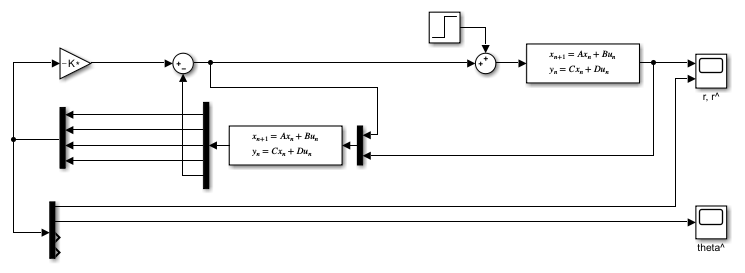
\includegraphics[width=\linewidth]{asset/d^.png}
        \end{center}

        Az állapotbecslőnél már megismert módot tudunk kiindulni és ugyanazt az eredményt kapjuk, kivéve az alábbi változtatásokat ($D = 0$ feltételezve):
        \begin{align}
            (\Phi, \Gamma, C) & \mapsto (\tPhi, \tGamma, \tC) \\
            x_k & \mapsto \hat{\tx}_k = 
            \begin{pmatrix}
                \hat{x}_k \\
                \hat{d}_k
            \end{pmatrix}
        \end{align}
        A változtatásokat végrehajtva a következő állapotegyenlet leírást kapjuk az új állapotbecslőre:
        \begin{align}
            \hat{\tx}_{k+1} & = F \hat{\tx}_k +
            \begin{bmatrix}
                H & G
            \end{bmatrix}
            \begin{pmatrix}
                u_k \\
                y_k
            \end{pmatrix} \\
            & = F \hat{\tx}_k + H'u'
            \\
            y_k^{\textrm{becslő}} & = \Eye \hat{\tx}_{k} + \ZerosV u'
        \end{align}

\section{Alapjel figyelembevétele}
    Az eddig látott megoldások mind az első rendszer által megvalósított csillapításra épültek rá, így a rendszer állapota végül mindig 0-ba lett irányítva. Azonban cél lehet, hogy általunk kívánt értéket vegyen fel a rendszer, mégpedig annak kimenetén, hiszen szemantikailag ez az amit a rendszerből kívánunk látni, illetve ezt tudjuk hatékonyan mérni. Ezt a kívánt kimeneti értéket nevezzük alapjelnek és $r$-rel jelöljük.

    Az alapjel előállításához a következő sémát használhatjuk:
    \begin{center}
        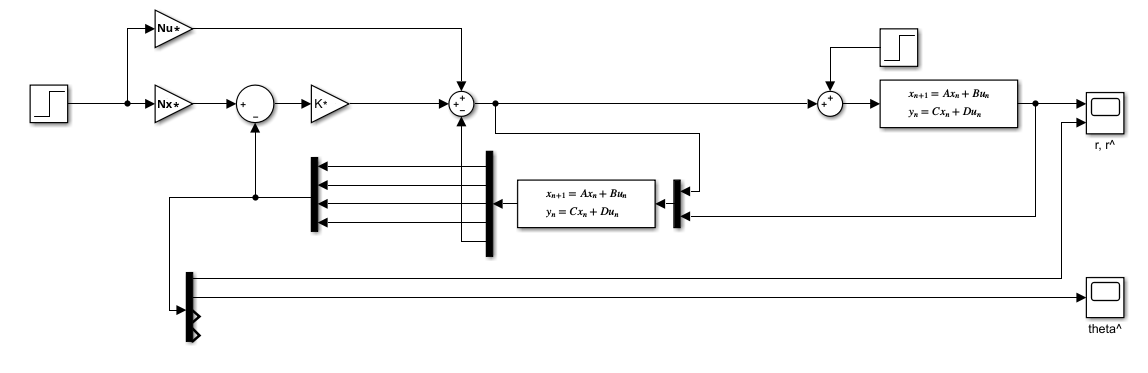
\includegraphics[width=\linewidth]{asset/N.png}
    \end{center}
    Bár a sémát a legutolsó rendszerre lett illesztve az ábrán, illetve az elkövetkező számolásokban is a legutolsó rendszert feltételezzük, azonban az bármelyik előző rendszerre is ráilleszthető.

    Látható, hogy $Nx$ és a kivánt kimenet szorzata meghatározza a kívánt állapotvektort. Ha a kívánt állapotvektort eltoljuk a jelenlegi (becsült) állapotvektorral, akkor a rendszerünk számára egy új origót határozunk meg, így az új origó felé való konvergáláskor valójában a kívánt állapotvektort felé fog konvergálni. %\todo{Nu-ra miért van szükség}
    Így az új bemenet a következő képpen néz ki:

    \newcommand{\nx}{\vec{N}_x}
    \begin{align}
        u = -K(\nx r_k - \hat{\tx}_k) + N_u r_k - \hat{d}_k
    \end{align}

    $\nx$ és $N_u$ meghatározásához felhasználjuk, hogy a cél az, hogy a kívánt állapotvektor és a jelenlegi (becsült) állapotvektor között ne legyen különbség bizonyos idő $(\infty)$ elteltével, ezért:
    \begin{align}
        r_\infty & = y_\infty
    \end{align}
    \begin{align}
        \tx_\infty = \hat{\tx}_\infty
    \end{align}
    \begin{align}
        \nx r_\infty - \hat{\tx}_\infty & = 0 \\
        \hat{\tx}_\infty & = \nx r_\infty \\
        \tx_\infty & = \nx r_\infty
    \end{align}
    \begin{align}
        u_\infty & = N_u r_\infty
    \end{align}
    Ezeket az egyenlőségeket felhasználva a rendszerünk állapotegyenleteit $\infty$ időben ($D = 0$-t feltételezve) felírva megkapjuk $\nx$-et és $N_u$-t:
    \begin{align}
        \nx r_\infty & = \tPhi \nx r_\infty + \tGamma N_u r_\infty \\
        r_\infty & = \tC \nx r_\infty
    \end{align}
    \begin{align}
        \nx & = \tPhi \nx + \tGamma N_u \\
        1 & = \tC \nx
    \end{align}
    \begin{align}
        \begin{pmatrix}
            \nx \\
            N_u
        \end{pmatrix} & =
        \begin{bmatrix}
            \tPhi - \Eye & \tGamma \\
            \tC          & 0
        \end{bmatrix}^{-1}
        \begin{pmatrix}
            \ZerosV \\
            1
        \end{pmatrix}
    \end{align}
    
\section{Két rendszer összekapcsolása}
    Végül az eredeti rendszert összekapcsoljuk egybe, amit egy $\left(\begin{smallmatrix}r \\ l\end{smallmatrix}\right)$ vektorral tudunk irányítani

    \begin{minipage}{\linewidth}
        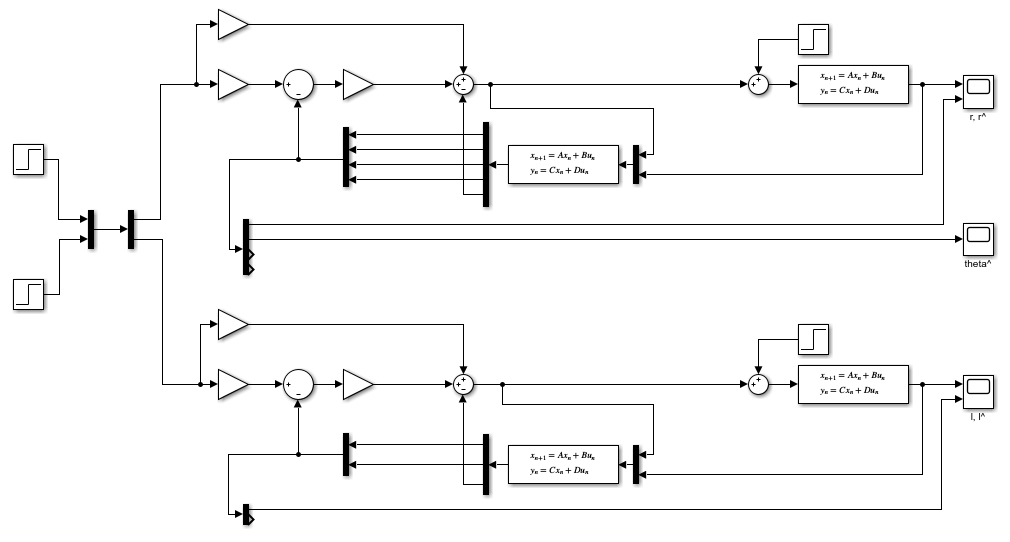
\includegraphics[width=\linewidth]{asset/rl.png}
        \captionof{figure}{control.slx}
    \end{minipage}

\section{Szabályozási eredmények}
    Szabályzás során a következő alapjelek lettek felhasználva:
    \begin{align}
        r_a & =
        \begin{cases*}
            2 & ha $t \geq 6$ \\
            0   & 
        \end{cases*} \\
        l_a & =
        \begin{cases*}
            4 & ha $t \geq 8$ \\
            0   & 
        \end{cases*}
    \end{align}
    A jelekre ható zavarás pedig:
    \begin{align}
        d_r & =
        \begin{cases*}
            5 & ha $t \geq T_{d,\textrm{start}}$ \\
            0   & 
        \end{cases*} \\
        d_l & =
        \begin{cases*}
            3 & ha $t \geq T_{d,\textrm{start}}$ \\
            0   & 
        \end{cases*}
    \end{align}

    Ezek hatására a következő az $r, \vartheta, l$ értékei:
    \begin{center}
        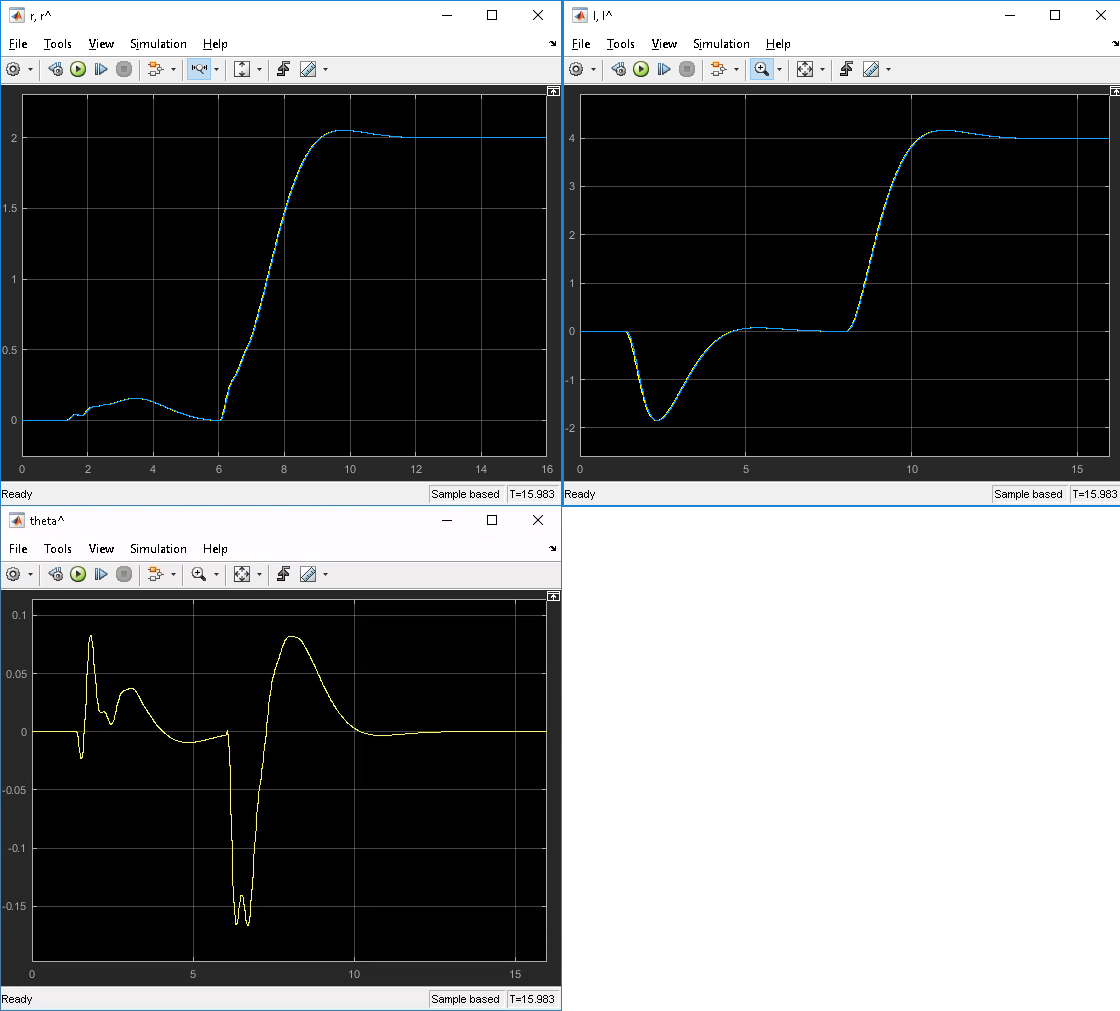
\includegraphics[width=\linewidth]{asset/result.png}
    \end{center}
    Látható, hogy a rendszer eleinte próbál 0-ba tartani, azonban $t = T_{d,\textrm{start}}$-ban a zaj kitéríti a rendszert. $t = 6$-ban, illetve $t = 8$-ban látható, hogy a rendszer közel van a 0 értékhez, azonban ekkor megváltozik az alapjel, és ezután a rendszert az új alapjeleket fogja követni rövidesen a kimenetén.

\section{Feladat általi szabályzás eredményei}
    Ezután frissítettem a Simulink modellt, hogy a feladat által kért szabályozást valósítsa meg. A feladat kiírása szerint módosítottam $T_{d, \textrm{start}}$-ot, hogy ne lapolódjanak át a tranziensek, így végül $t = 4$-kor lép csak be a zaj. Szintén módosítottam $d_{norm}$-ot, az alapján, hogy $d_{norm} = 1$ esetén mekkor volt a kitérés mértéke $(\approx0.3 - 0.09)$. Így végül $d_{norm}$ értéke $0.4286$ lett, ami által közel egyező lett az eltérések mértéke:

    \begin{center}
        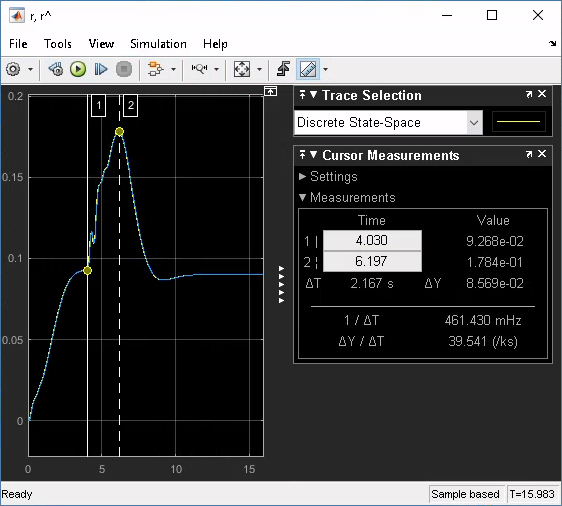
\includegraphics[width=\linewidth*2/3]{asset/diff.png}
    \end{center}

    \begin{minipage}{\linewidth}
        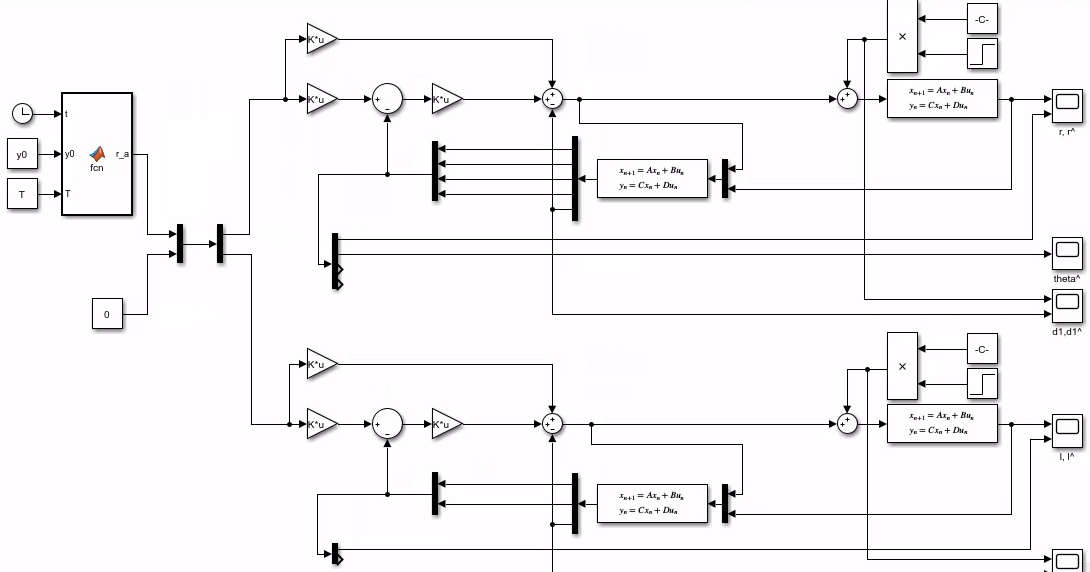
\includegraphics[width=\linewidth]{asset/rl2.png}
        \captionof{figure}{control2.slx}
    \end{minipage}

    \begin{center}
        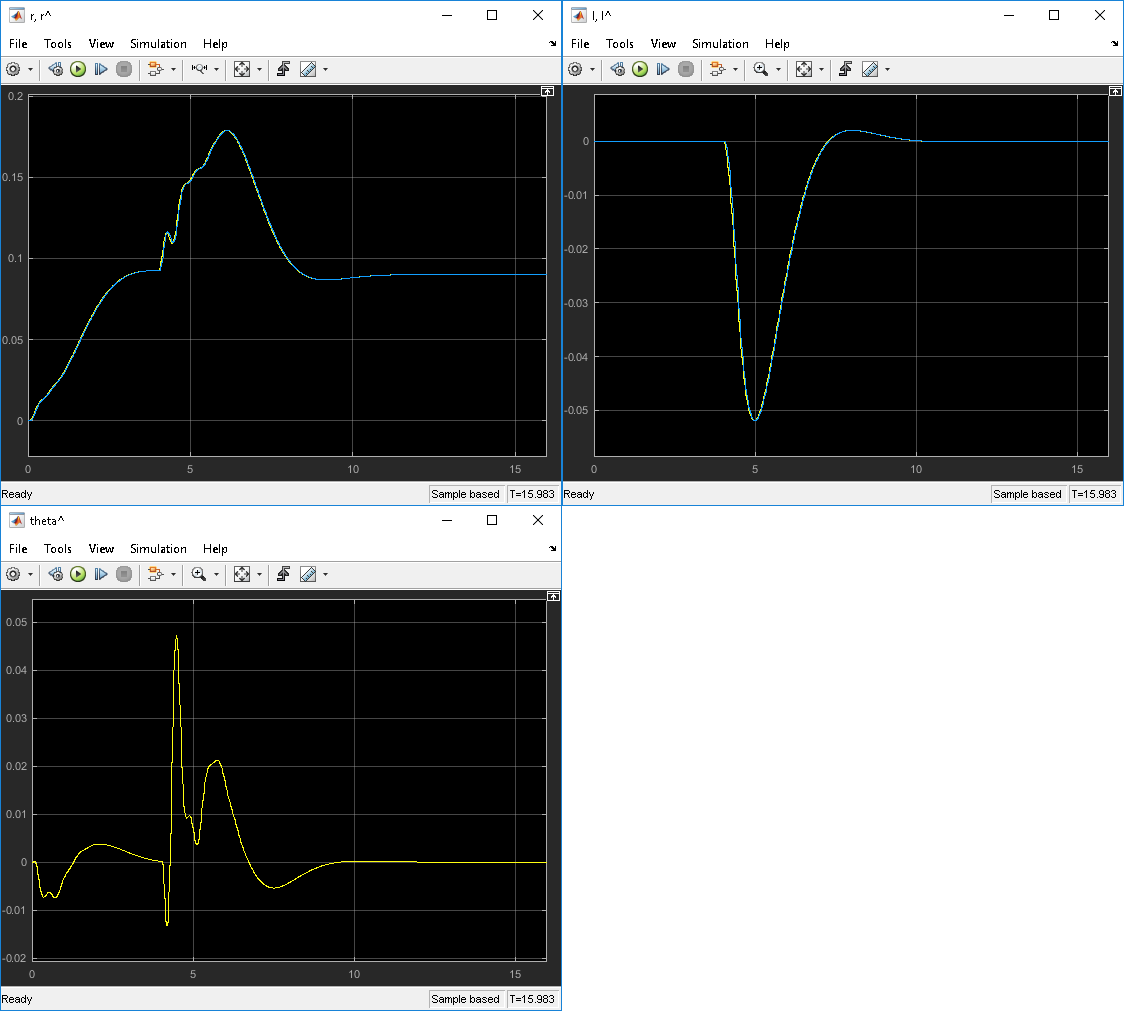
\includegraphics[width=\linewidth]{asset/result2.png}
    \end{center}


\end{document}